\documentclass[xcolor=svgnames]{beamer} 
\setbeamertemplate{caption}{\raggedright\insertcaption\par}
\usepackage[utf8]{inputenc}
\usepackage{xcolor}
\usepackage{booktabs, comment} 
\usepackage{pgfpages}
\usepackage{csquotes}
\usepackage{amsmath}
\usepackage{tikz}
\usetheme{Madrid}
\usepackage[version=4]{mhchem}
\usepackage{adjustbox}
\usepackage{tikz}
\usepackage{tikzlings}
\usetikzlibrary{decorations.pathmorphing,arrows.meta}
\usepackage{cancel}

% COLORS 
\definecolor{mqred}{RGB}{166, 25, 46}
\definecolor{mqdeepred}{RGB}{118, 35, 47}
\definecolor{mqgray}{RGB}{55, 58, 54}
\definecolor{mqlightgray}{RGB}{237, 235, 229}
\definecolor{mqmagenta}{RGB}{198, 0, 126}
\usecolortheme[named=mqred]{structure}
\setbeamercolor{title in head/foot}{bg=mqlightgray, fg=mqgray}
\setbeamercolor{author in head/foot}{bg=mqdeepred}
\setbeamercolor{page number in head/foot}{bg=mqdeepred, fg=mqlightgray}
\usefonttheme[onlymath]{serif}

% FOOTNOTE ARRANGEMENTS

\makeatletter
\setbeamertemplate{footline}{
  \leavevmode%
  \hbox{%
  \begin{beamercolorbox}[wd=.5\paperwidth,ht=2.25ex,dp=1ex,center]{author in head/foot}%
    \usebeamerfont{author in head/foot}\insertshortauthor\expandafter\ifblank\expandafter{\beamer@shortinstitute}{}{~~(\insertshortinstitute)}
  \end{beamercolorbox}%
  \begin{beamercolorbox}[wd=.4\paperwidth,ht=2.25ex,dp=1ex,center]{title in head/foot}%
    \usebeamerfont{title in head/foot}\insertshorttitle
  \end{beamercolorbox}%
  \begin{beamercolorbox}[wd=.1\paperwidth,ht=2.25ex,dp=1ex,center]{page number in head/foot}%
    \usebeamerfont{page number in head/foot}\insertframenumber{} / \inserttotalframenumber 
  \end{beamercolorbox}}%
  \vskip0pt%
}
\makeatother
\beamertemplatenavigationsymbolsempty


% TITLE, AUTHORS, INSTITUTE, DATE

\title[Sympathetic Cooling Optimization]{Sympathetic Cooling Optimization for Precision Spectroscopy of Chiral Molecular Ions}
\author{Doron Behar}
\institute[Yuval Shagam's Group]{Technion Institute of Technology / Solid State Institute}
\date{\today}

% LOGO
\titlegraphic{
\includegraphics[width=0.8\linewidth]{graphics/logo.pdf}} % Change the logo path as needed

\begin{document}

\begin{frame}
    \titlepage
\end{frame}

% Section and Frame examples
\section{Introduction}
\subsection{Motivation}
\subsubsection{In General}
\begin{frame}{About Chiral Molecules}{What are They?}

Chiral = 'Handedness' (Greek)

\begin{columns}
\begin{column}{.6\textwidth}
\begin{figure}
    \centering
    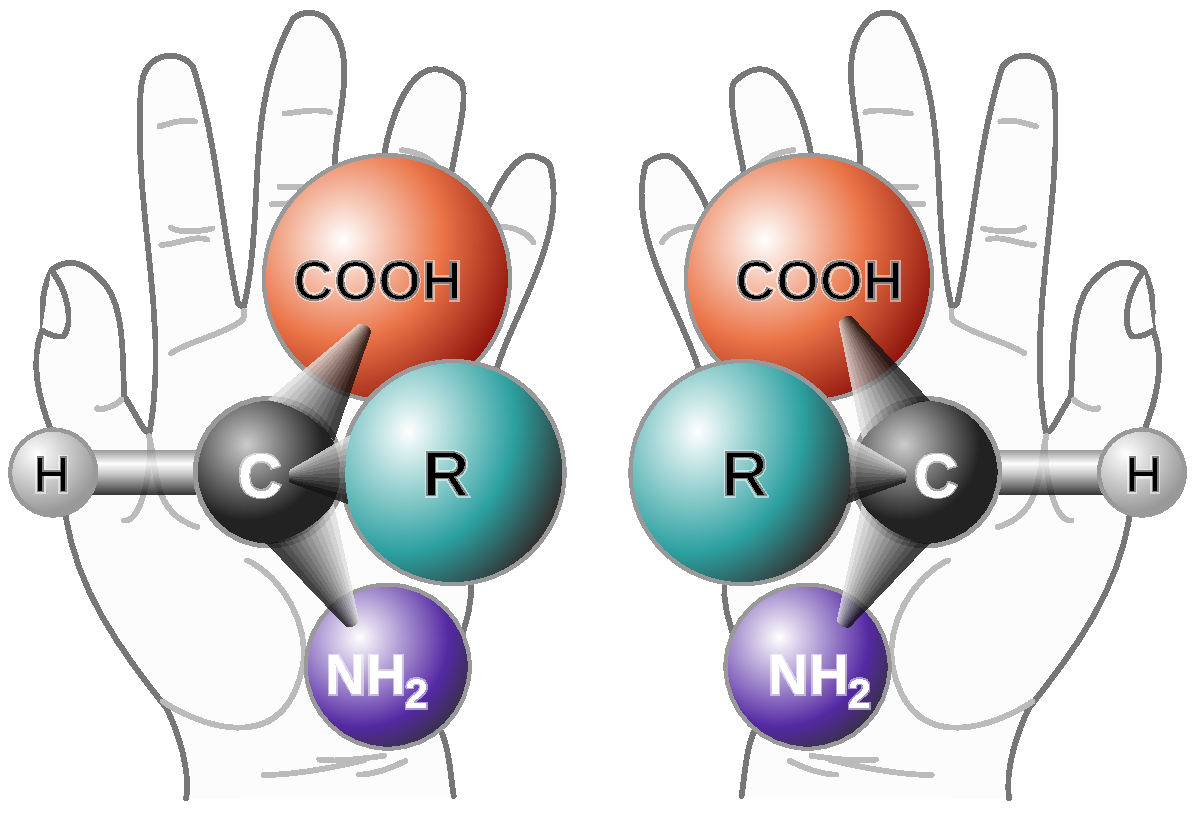
\includegraphics[width=\linewidth]{graphics/chirality_with_hands.pdf}
\end{figure}
\end{column}
\begin{column}{.3\textwidth}
\only<2>{
\begin{figure}
    \centering
    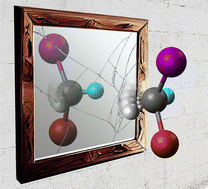
\includegraphics[width=\linewidth]{graphics/broken-symmetry.png}
\end{figure}
}
\end{column}%
\end{columns}

\end{frame}

\begin{frame}{About Chiral Molecules}{Examples in the wild}

\begin{columns}
\begin{column}{.33\textwidth}
\only<2->{
\begin{figure}
    \centering
    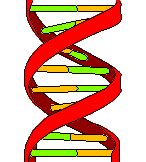
\includegraphics[width=\linewidth]{graphics/DNA.pdf}
\end{figure}
}
\end{column}
\begin{column}{.165\textwidth}
\only<3->{
Limonene
\begin{figure}
    \centering
    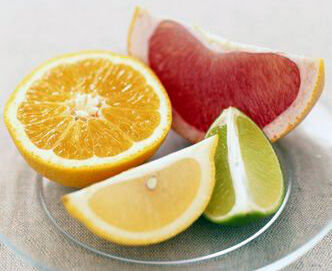
\includegraphics[width=\linewidth]{graphics/Limonane-fruits.jpg}
\end{figure}
}
\end{column}
\begin{column}{.165\textwidth}
\only<3->{
    % TODO: Check it looks OK
Caraway \tiny{German/Yiddish: Kummel}
\begin{figure}
    \centering
    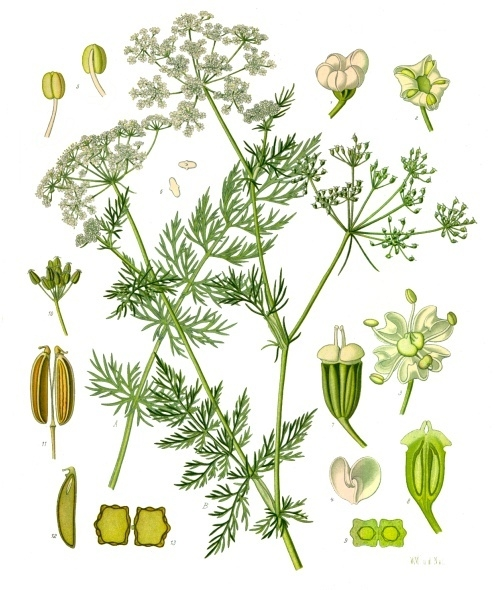
\includegraphics[width=\linewidth]{graphics/Caraway.jpg}
\end{figure}
}
\end{column}
\begin{column}{.33\textwidth}
\only<4->{Turnbuckle / Stretching-Screw
\begin{figure}
    \centering
    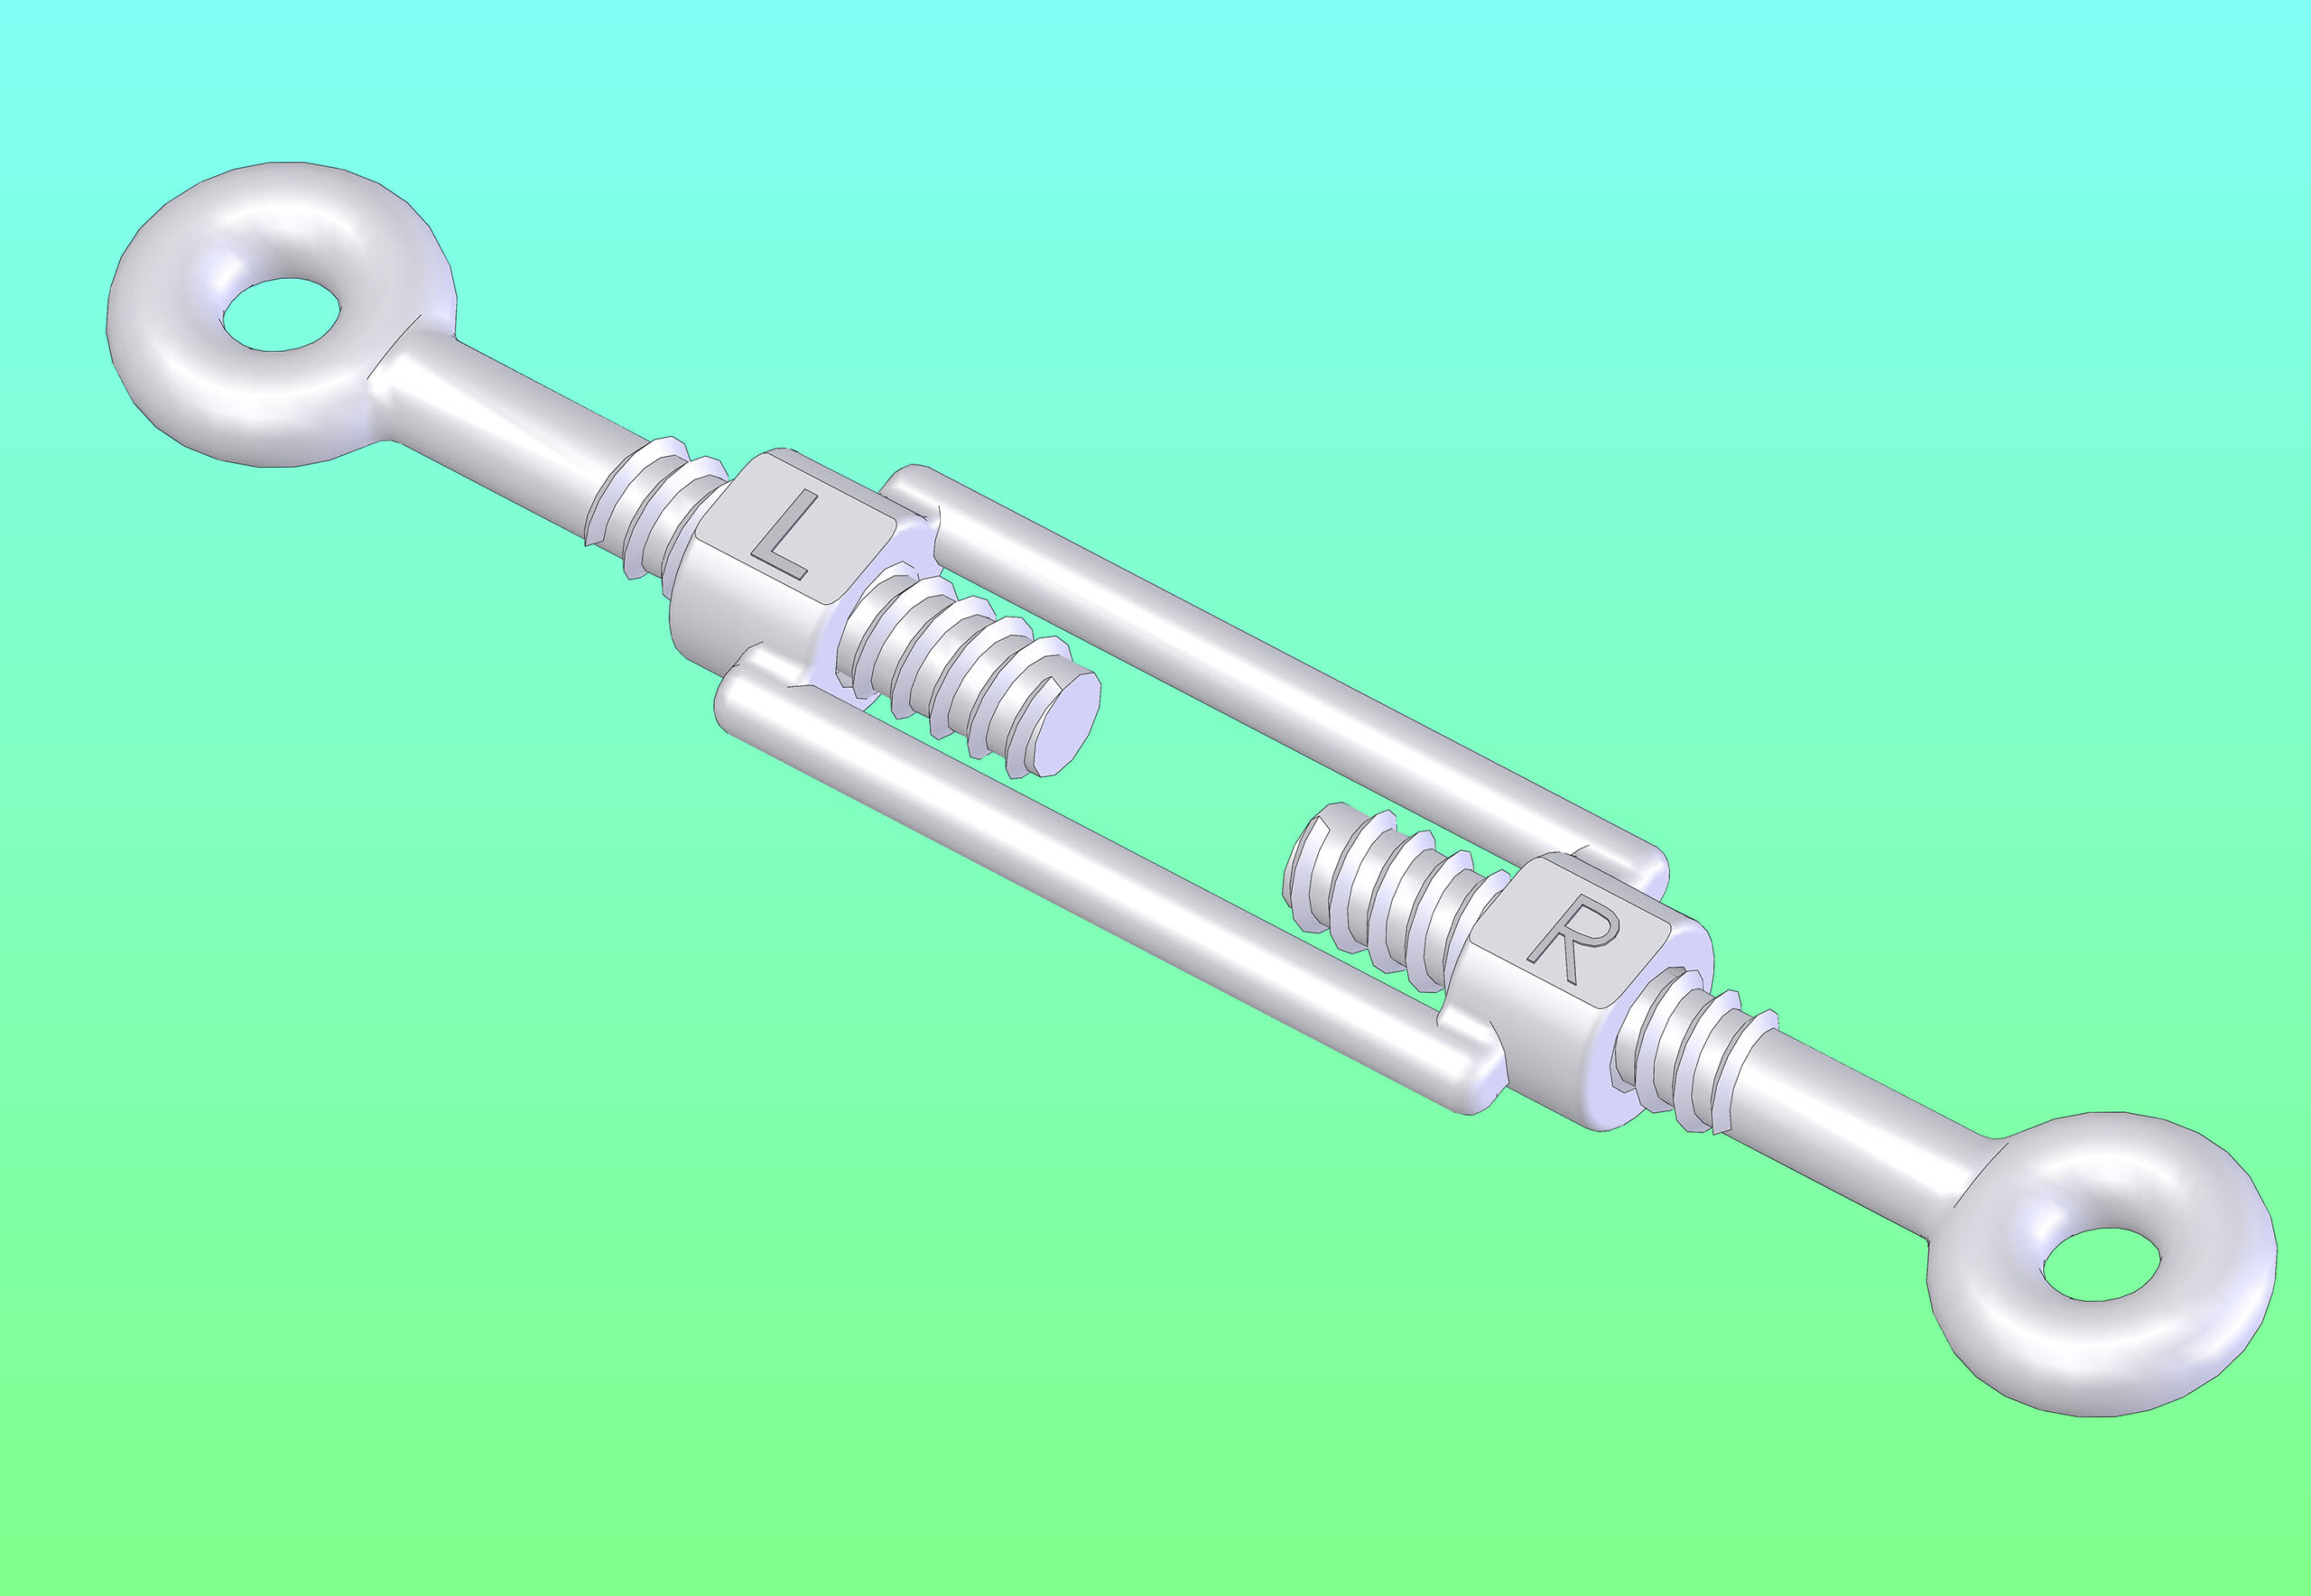
\includegraphics[width=\linewidth]{graphics/turnbuckle.png}
\end{figure}
}
\end{column}
\end{columns}

\end{frame}

\begin{frame}{Chirality Effects}
\begin{columns}
\begin{column}{.5\textwidth}
\only<1->{
Light Polarization
\begin{figure}
    \centering
    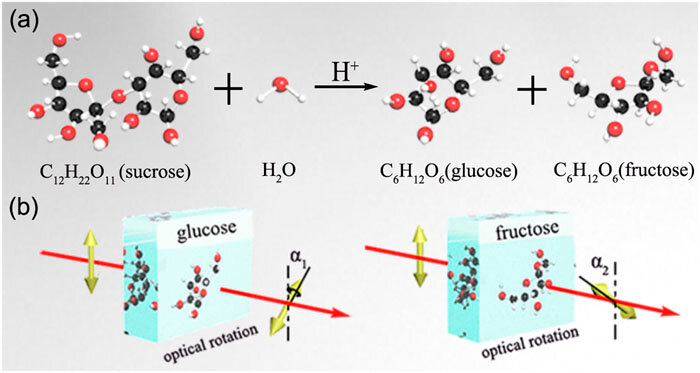
\includegraphics[width=\linewidth]{graphics/sugar-chirality.png}
\end{figure}
}
\end{column}
\begin{column}{0.5\textwidth}
\uncover<2->{
Molecular Vibration
\begin{figure}
    \centering
    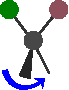
\includegraphics[width=0.5\linewidth]{graphics/molecular-wag-vibration.pdf}
\end{figure}
}
\uncover<4->{$\nu_\mathrm{vib} \approx 33.3\ \mathrm{THz}$, $\Delta_\mathrm{PV} \approx 1.8\ \mathrm{Hz}$}
\uncover<3->{
\begin{figure}
    \centering
    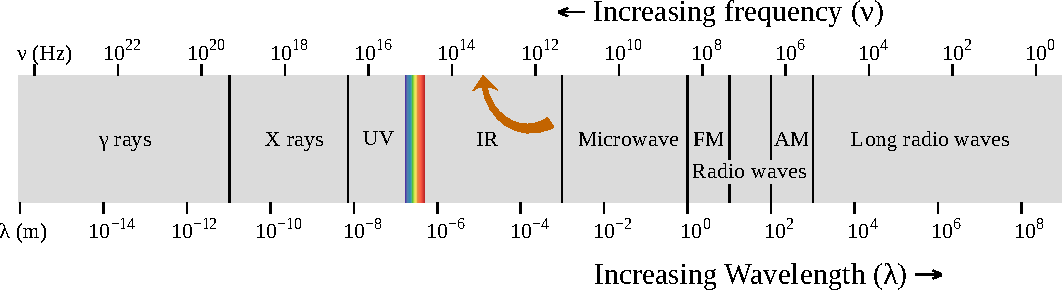
\includegraphics[width=\linewidth]{graphics/EM_spectrum_wide.pdf}
\end{figure}
}
\end{column}
\end{columns}
\end{frame}

\subsubsection{Researching Cooling}
\begin{frame}{Why Cooling?}{Reduce (Relativistic) Doppler Effect}

\begin{equation*}
    \uncover<2->{f_r - f_s = f_s \left(\sqrt{\frac{1-\beta}{1 + \beta}} - 1\right)}\uncover<3->{= f_s \left(-\beta + \frac{1}{2} \beta^2 + \mathcal{O}(\beta^3)\right)}\uncover<4->{,\ \beta^2 \simeq \frac{K_\mathrm{B}T}{mc^2}}
\end{equation*}
\begin{equation*}
\uncover<5->{f_s \approx 33.3\ \mathrm{THz},\ m = 222 \mathrm{AMU},\ |f_s - f_r| \overset{!}{<} \Delta_\mathrm{PV} \approx 1.8\ \mathrm{Hz}}
\end{equation*}
\uncover<6->{\begin{itemize}
    \item $ |f_s -f_r| \simeq 680\ \mathrm{kHz}/\sqrt{\mathrm{Kelvin}}$ (1st order)
    \item \uncover<7->{$ |f_s -f_r| \simeq 13\ \mathrm{mHz}/\mathrm{Kelvin}$ (2nd order)}
\end{itemize}}

\end{frame}

\begin{frame}{Why Cooling?}{Increase Coherence Time}
\begin{columns}
\begin{column}{.5\textwidth}
\uncover<1->{
Avoid Thermal Decoherence
\begin{figure}
    \centering
    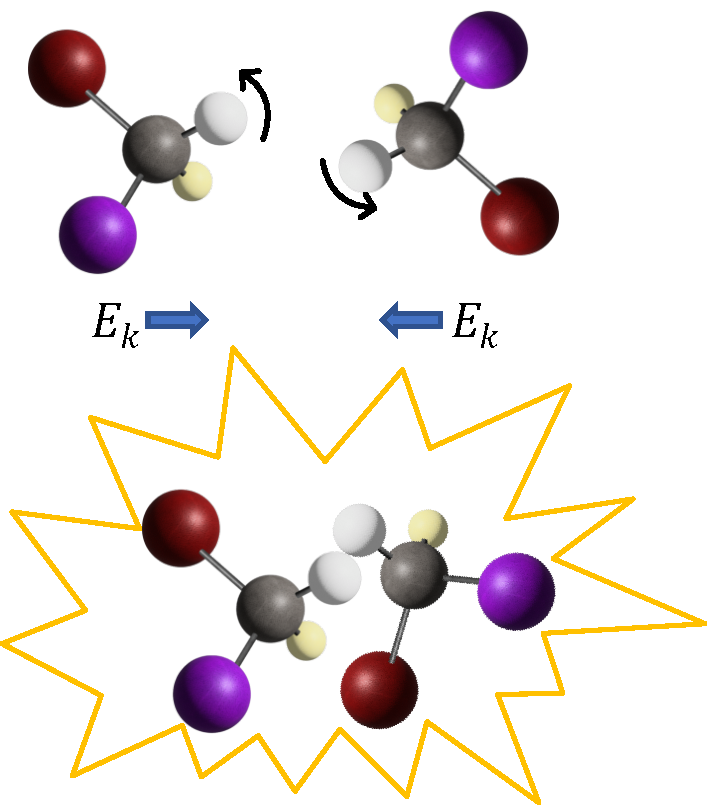
\includegraphics[width=\linewidth]{graphics/Decoherence.pdf}
\end{figure}
}
\end{column}
\begin{column}{0.5\textwidth}
\uncover<2->{In ion crystals coherence is maximal
\begin{figure}
    \centering
\adjincludegraphics[
    width=\linewidth,%
    trim={{.3\width} {.1\height} {.2\width} {.1\height}},%
    clip%
]{graphics/ion-crystal-example.pdf}
\end{figure}
}
\end{column}
\end{columns}
\end{frame}

\begin{frame}{Why Cool Fast?}
\begin{columns}

\begin{column}{.5\textwidth}
\begin{itemize}
    \uncover<1->{\item Ramsey-scheme works only for ground-state ionized molecule} % 
    \uncover<2->{\item Vaccum Chamber Black Body Radiation heats molecule internally}
    \uncover<3->{\item Our Ramsey-scheme (intentionally) dissociates the molecule}
    \uncover<4->{\item[$\Rightarrow$] \textbf{Molecules must be cooled fast internally \& externally}}
\end{itemize}
\end{column}
\begin{column}{0.5\textwidth}
\only<1>{
\begin{figure}
    \centering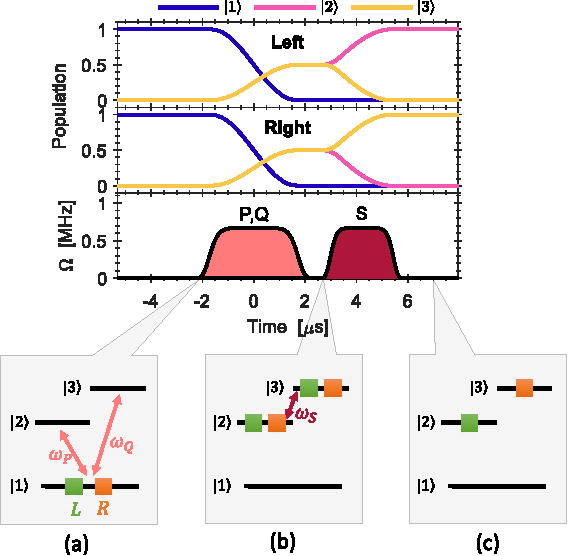
\includegraphics[width=\linewidth]{graphics/Ramsey-scheme-short.pdf}
\end{figure}
}
\only<2>{
\begin{figure}
    \centering\adjincludegraphics[
    width=\linewidth,%
    trim={{.523\width} 0 0 0},%
    clip%
]{graphics/experimental-system.pdf}
\end{figure}
}
\only<3->{
\begin{figure}
    \centering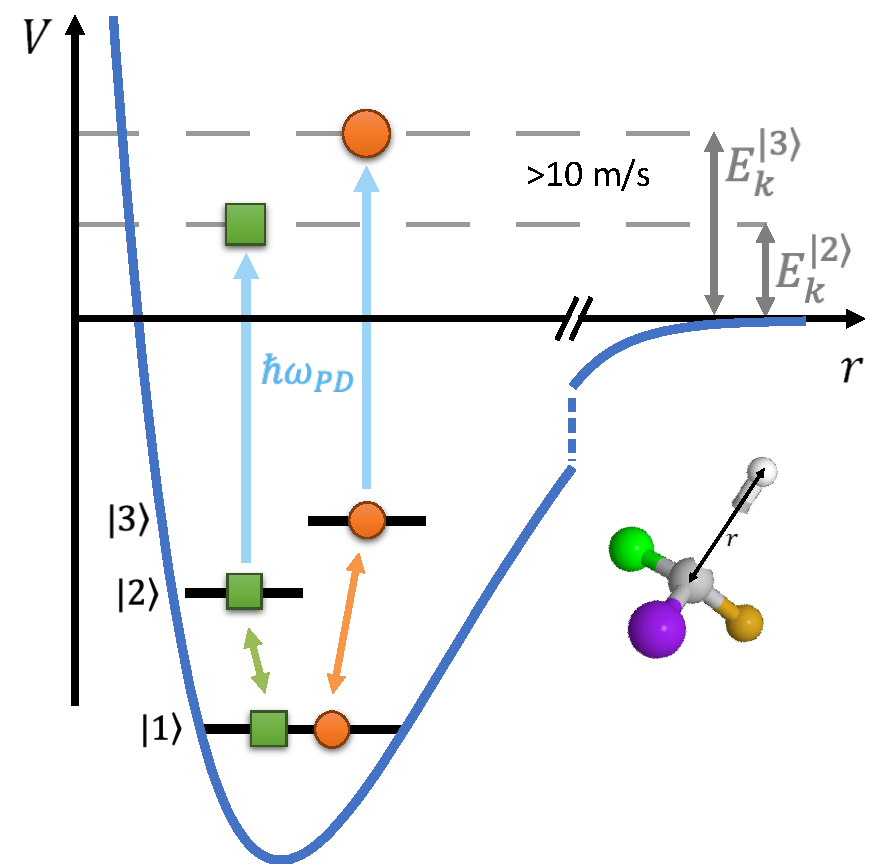
\includegraphics[width=\linewidth]{graphics/Ramsey-Dissociation.pdf}
\end{figure}
}
\end{column}

\end{columns}
\end{frame}

% TODO: Consider adding a frame comparing the cooling requirements to other cold ions users requirements - Like Ziv Meir, Pit Schmidt, Fabian Wolf etc.

\begin{frame}{How Fast \& Cold?}
\begin{itemize}
    \uncover<2->{\item Black body radiation decoheres molecules after $\approx 10\ \mathrm{s}$}
    \uncover<3->{\item Experiment's sequence frequency is $10\ \mathrm{Hz}$}
    \uncover<4->{\item Large statistics improves accuracy by $\sqrt{N}$}
    \uncover<5->{\item Faster cooling $\Rightarrow$ Larger $\frac{\mathrm{d}{N}}{\mathrm{d}t}$ $\Rightarrow$ Higher accuarcy}
    \uncover<6->{\item[!] Cold enough for our VMI's resolution}
\end{itemize}
% TODO: Consider putting an image of the experiment 10Hz sequence
% \only<3>{}...
\visible<4-5>{$$\begin{array}{ll}
T = \sum_i^N x_i & \mathrm{Var}(T) = \sum_i^N \mathrm{Var}(x_i) = N\sigma^2 \\
\bar{x} = T/n & \mathrm{Var}(\bar{x}) = \mathrm{Var}\left(\frac{T}{n}\right) = \frac{1}{N^2}\mathrm{Var}(T) = \frac{\sigma^2}{N}
\end{array}$$}
\visible<6>{
\vspace{-3em}
\begin{figure}
    \centering
    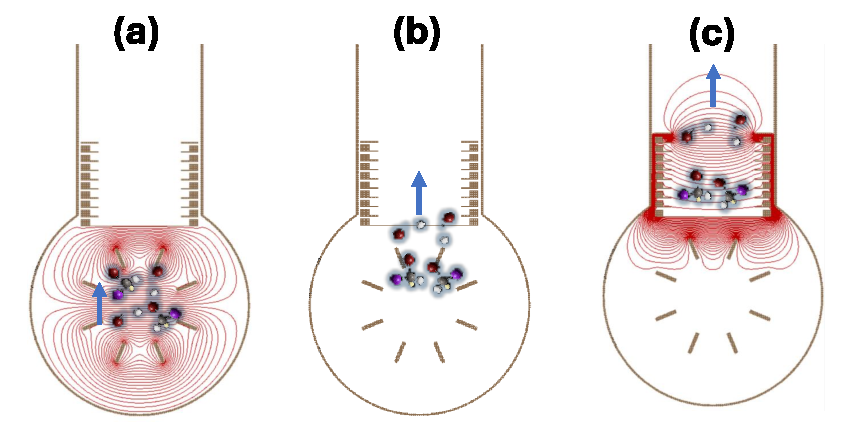
\includegraphics[width=0.7\linewidth]{graphics/trapping-and-VMI.pdf}
\end{figure}
}
\end{frame}

\subsection{Theory}
\begin{frame}{Theory: LASER Cooling Model}{Bloch Equations}
\begin{equation*}
\uncover<2->{\mathcal{H}_0 = \frac{p^2}{2m} + \frac{1}{2}m\omega_0^2 x^2 = \hbar \omega_0 \left(a^\dagger a +\frac{1}{2}\right)}\uncover<3->{,\ \mathcal{H}_\mathrm{AF} = -\mathbf{d}\cdot\mathbf{E}}
\end{equation*}
\begin{equation*}
    \uncover<4->{\mathcal{H} = \mathcal{H}_0 + \mathcal{H}_\mathrm{AF}}\uncover<5->{,\ \partial_t \rho = \frac{i}{\hbar}[\mathcal{H}, \rho]}\uncover<6->{+ \Gamma D[a]\rho}
\end{equation*}
\begin{equation*}
\uncover<6->{D[a]\rho \equiv a\rho a^\dagger - \frac{1}{2}\{a^\dagger a, \rho\}\equiv \text{Lindbland super operator}}
    % Say when uncovering 5: The Lindblandian is responsible for the interaction of the atom with the vaccum - like in other open quantum systems. \gamma is the dumping due to that.
\end{equation*}
\begin{equation*}
\uncover<7->{\mathbf{F} = \partial_t \mathbf{p} = \frac{i}{\hbar}[\mathcal{H},\mathbf{p}]}\uncover<8->{,\ \text{RWA}\ldots\Rightarrow \left\langle\mathbf{F}_\mathrm{rad}\right\rangle = \Gamma \rho_\mathrm{ee}(t\rightarrow\infty)\hbar \mathbf{k}}
\end{equation*}
\begin{equation*}
    \uncover<9->{\boxed{\left\langle\mathbf{F}_\mathrm{rad}\right\rangle(\mathbf{v}) =  \frac{h \Gamma \hat{k}}{2\lambda} \cdot \frac{\Omega^2/2}{\Gamma^2/4 + \Omega^2/2 + (\delta -\mathbf{k}\cdot\mathbf{v})^2}}}
\end{equation*}
\uncover<10->{\tiny{Derivation from: Dan Steck - \textit{Quantum and Atom Optics}}}
\end{frame}

\begin{frame}{LASER Cooling Force Properties}{A Classical View}
\small{For simplicity: $\hat{k} = (1,0,0), \mathbf{v}=(v,0,0)$}
\begin{columns}
\begin{column}{.5\textwidth}
\begin{equation*}
    \uncover<2->{\left\langle\mathbf{F}_\mathrm{rad}\right\rangle(\mathbf{v})= F_0 \hat{x}\left(\alt<6->{\cancel{1 + }}{1 +}\alt<6->{\ 2\cdot}{}\frac{\partial F}{\partial v}\cdot v + \mathcal{O}(v^2) \right)}
\end{equation*}
\uncover<3->{Force in a Harmonic Oscillator:
$$\ddot{x} = \omega^2 x + \alt<7->{\cancel{F_0/m}}{F_0/m} - 2\xi \omega \dot{x} + \mathcal{O}\left(\dot{x}^2\right)$$
}
\uncover<4->{
$$x(t) = \alt<8->{\cancel{\frac{F_0}{m \omega^2}}}{\frac{F_0}{m \omega^2}} + x_0 e^{-\xi\omega t} \sin\left(\tilde{\omega} t + \phi \right)$$
}

\end{column}
\begin{column}{.5\textwidth}
\begin{figure}
\centering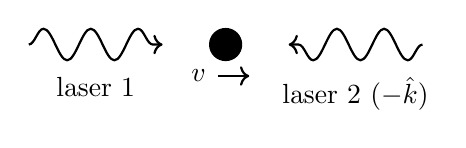
\begin{tikzpicture}
  % Left laser (Laser 1)
  \visible<2->{\draw[->,decorate,decoration={snake,amplitude=2mm,segment length=6mm},thick] 
    (-2.5,0) -- (-0.8,0) node[midway, below=8pt] {laser 1};}
  % Right laser (Laser 2)
  \visible<5->{\draw[->,decorate,decoration={snake,amplitude=2mm,segment length=6mm},thick] 
    (+2.5,0) -- (+0.8,0) node[midway, below=8pt] {laser 2 $(-\hat{k})$};}
  % Particle (black circle)
  \fill (0,0) circle (6pt);
  % Particle Velocity arrow
  \draw[->,thick] (-0.1,-0.4) -- (0.3,-0.4) node[left=12pt] {$v$};
\end{tikzpicture}
\end{figure}
\visible<9->{\begin{figure}
    \centering
    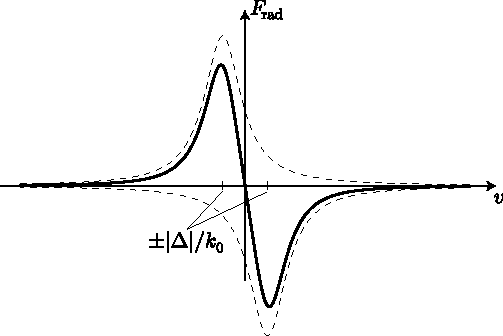
\includegraphics[width=\linewidth]{graphics/LASER-cool-force-oddity.pdf}
\end{figure}}
\end{column}
\end{columns}
\end{frame}

\begin{frame}{Ion Trapping}{The Basics}
\uncover<2->{Problem: Laplace equation: $\nabla^2\phi = 0$}

\begin{columns}

\begin{column}{0.25\textwidth}
\uncover<3->{\begin{figure}
    \centering
    \alt<3-9>{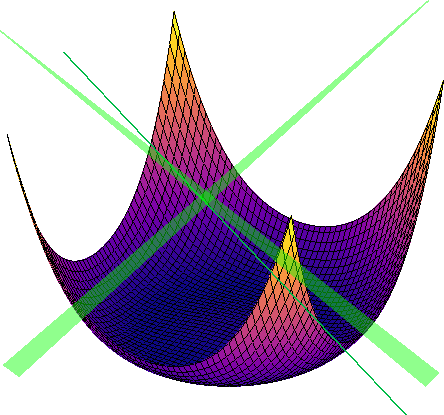
\includegraphics[width=\linewidth]{graphics/ion-trap-basics@effective.pdf}}{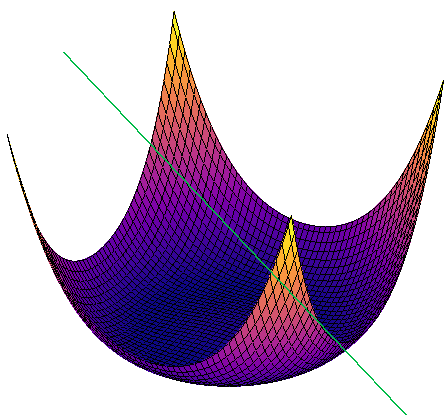
\includegraphics[width=\linewidth]{graphics/ion-trap-basics@effectiveNoX.pdf}}
    \caption{\uncover<10->{Effective}}
\end{figure}}
\end{column}

\begin{column}{0.25\textwidth}
\uncover<4->{\begin{figure}
    \centering
    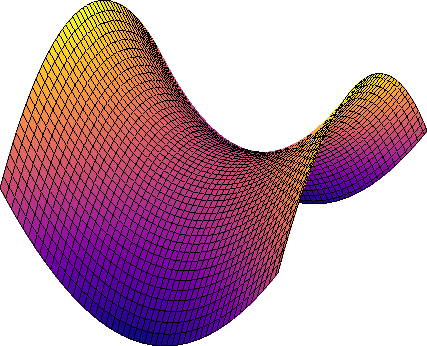
\includegraphics[width=\linewidth]{graphics/ion-trap-basics@0.pdf}
    \caption{\uncover<8->{$f_\mathrm{rf} t=0$}}
\end{figure}}
\end{column}

\begin{column}{0.25\textwidth}
\uncover<9->{\begin{figure}
    \centering
    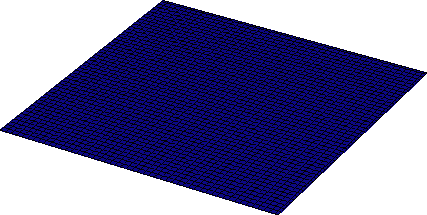
\includegraphics[width=\linewidth]{graphics/ion-trap-basics@PiOver2.pdf}
    \caption{$f_\mathrm{rf} t=1/4$}
\end{figure}}
\end{column}

\begin{column}{0.25\textwidth}
\uncover<5->{\begin{figure}
    \centering
    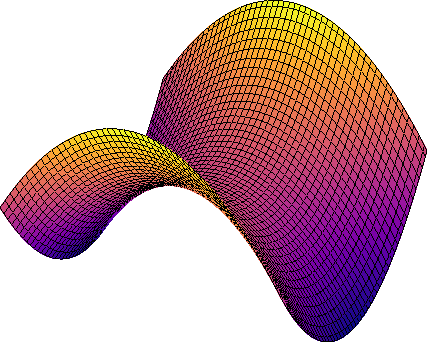
\includegraphics[width=\linewidth]{graphics/ion-trap-basics@Pi.pdf}
    \caption{\uncover<8->{$f_\mathrm{rf} t = 1/2$}}
\end{figure}}
\end{column}

\end{columns}

$$\uncover<6->{\phi = \sum_{i\in\{x,y,z\}} x_i^2 \left(a_i + q_i \cos(2\pi f_\mathrm{rf} t)\right)}\uncover<7->{,\ \sum_{i\in\{x,y,z\}} a_i = \sum_{i\in\{x,y,z\}} q_i = 0}$$
\end{frame}

\begin{frame}{Mathieu Equation: Introduction}
\uncover<2->{$$\phi = \sum_{i\in\{x,y,z\}} x_i^2 \left(a_i + q_i \cos(2\pi f_\mathrm{rf} t)\right) \Rightarrow \ddot{x}_i = \left(\tilde{a}_i + 2\tilde{q}_i\cos(2\tau)\right) x$$}
\uncover<3->{\begin{figure}
    \centering
    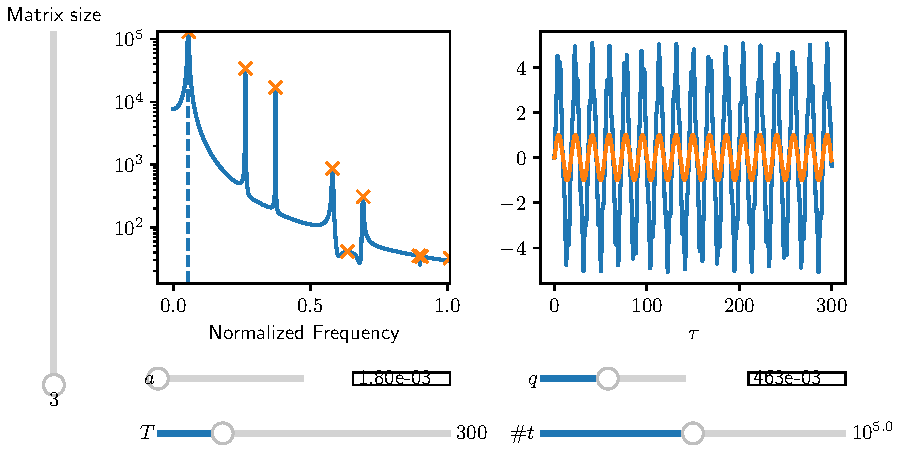
\includegraphics[width=0.8\linewidth]{graphics/pure-mathieu-fft.pdf}
    \caption{$\pi f_\mathrm{rf}t \equiv \tau\uncover<4->{,\ (\tilde{a}_i, \tilde{q}_i) \rightarrow f_\mathrm{sec}}\uncover<5->{\underset{\text{typically}}{\ll} f_\mathrm{rf}}$}
\end{figure}}

\end{frame}

\begin{frame}{Mathieu Equation Solved Reversely}
\begin{columns}

\begin{column}{0.4\textwidth}
$$(\tilde{a}_i, \tilde{q}_i) \rightarrow f_\mathrm{sec}$$
\uncover<2->{$$\begin{pmatrix}
    \tilde{a}_x & \tilde{q}_x \\
    \tilde{a}_y & \tilde{q}_y \\
    \tilde{a}_z & \tilde{q}_z \\
\end{pmatrix} \mathcolor{red}{\overset{\alt<2-4>{?}{}}{\leftarrow}} \begin{pmatrix}
    f_\mathrm{sec(x)} \\
    f_\mathrm{sec(y)} \\
    f_\mathrm{sec(z)}
\end{pmatrix}$$}
\uncover<3->{$$\begin{pmatrix}
    \sum_i \tilde{a}_i = 0 \\
    \sum_i \tilde{q}_i = 0 \\
    \uncover<4->{q_z= 0}
\end{pmatrix}$$}
\end{column}

\begin{column}{0.6\textwidth}
\uncover<5->{\begin{figure}
    \centering
    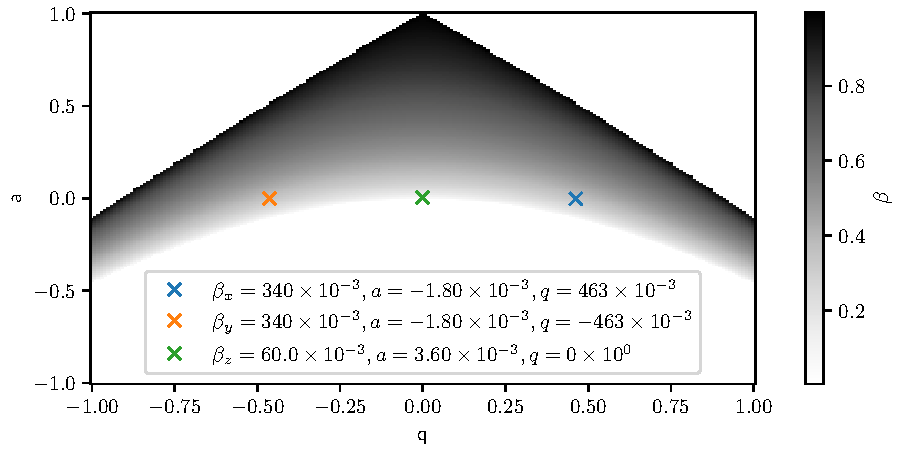
\includegraphics[width=\linewidth]{graphics/pure-mathieu-stability.pdf}
    \caption{\textit{Mathieu Stability Diagram}}
\end{figure}}
\end{column}

\end{columns}    
\end{frame}

\begin{frame}{Deviations from a Harmonic Trap}
\begin{columns}

\begin{column}{0.46\textwidth}
\uncover<2->{$$ \omega_\mathrm{sec(target)} = \omega_\mathrm{sec(cooler)}\sqrt{\frac{m_\mathrm{cooler}}{m_\mathrm{target}}} $$}
\uncover<3->{$$(\tilde{a},\tilde{q}) \propto \frac{1}{m_\mathrm{cooler}}$$}
\uncover<3->{$$\omega_\mathrm{sec(target)} \alt<4->{\leftarrow (a,q)\cdot\frac{m_\mathrm{cooler}}{m_\mathrm{target}}}{=?}$$}    
\end{column}

\begin{column}{0.54\textwidth}
\uncover<4->{\begin{figure}
    \centering
    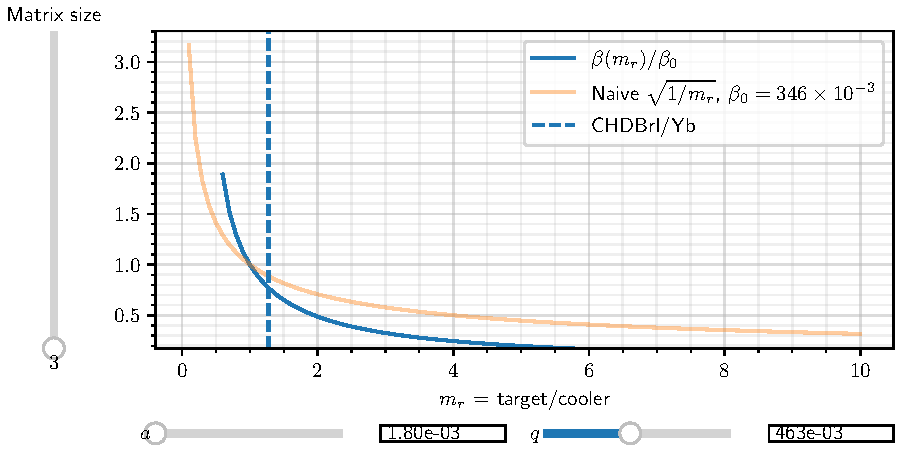
\includegraphics[width=\linewidth]{graphics/mathieu-mass-dep.pdf}
\end{figure}}
\end{column}

\end{columns}
\end{frame}

\section{Optimizing LASER parameters}

\begin{frame}{Preliminary LASER Cooling Adjustments}
Reminder:
\end{frame}

\begin{frame}
    \centering
    \textbf{Thank you!}\\
    Questions?
\end{frame}

\end{document}
